% Approach: combining CMB and time delay distances. Blinding.

% Results. Internal consistency. Consistency with other probes.

% Combination with stellar kinematics, introduces additional
% distance dependency. Not correlated, and weaker dependence than Ddt
% (See discussion with SHS about Jee et al papers)

Early approaches to inferring cosmological parameters from time delay
lens observations focused on measuring the Hubble constant in a
Friedman-Robertson-Walker model with asserted (fixed) density
parameters.\footnote{The original investigation by \citet{Ref64}
involved the ``assumption that the linear distance--red-shift relation
is valid.''} With better data came the recognition that time delay
lenses were really probes of cosmological distance
\citep{Koo++03,Suy++10}, and the emphasis shifted to
inferring the set of cosmological parameters that are needed  to predict
the kinematics of the expansion of the Universe out to the redshift of
the source.

The amount of cosmological information in an individual lens
is still relatively small, and the parameter most strongly constrained
is  the Hubble constant, but as sample sizes increase we expect
ensembles of  lenses to support the inference of several cosmological
parameters (or combinations thereof).

In Figure~\ref{fig:current-constraints} we reproduce the current best
constraints on  cosmological parameters, from the two best-measured
systems, B1608$+$656 and RXJ1131 \citep{Suy++14}. When this figure was
made, the available precision from just these two lenses was about the
same as that from SDSS DR7 BAO \citep{PercivalEtal2010} and the
``Constitution'' set of Type Ia supernovae \citep{HickenEtal2009}.
When all three of the curvature density $\Ok$, Dark Energy
density $\ODE$ and equation of state
$\wDE$ parameters are allowed to vary, along with $H_0$, we see that the
time delay lenses provide similar constraints to BAO and complementary
constraints to the SNe: the time delays and
the BAO signal depend on angular diameter distances and $H_0$, while
the supernovae probe luminosity distances.

%%%%%%%%%%%%%%%%%%%%%%%%%%%%%%%%%
\begin{figure*}[!ht]
\centering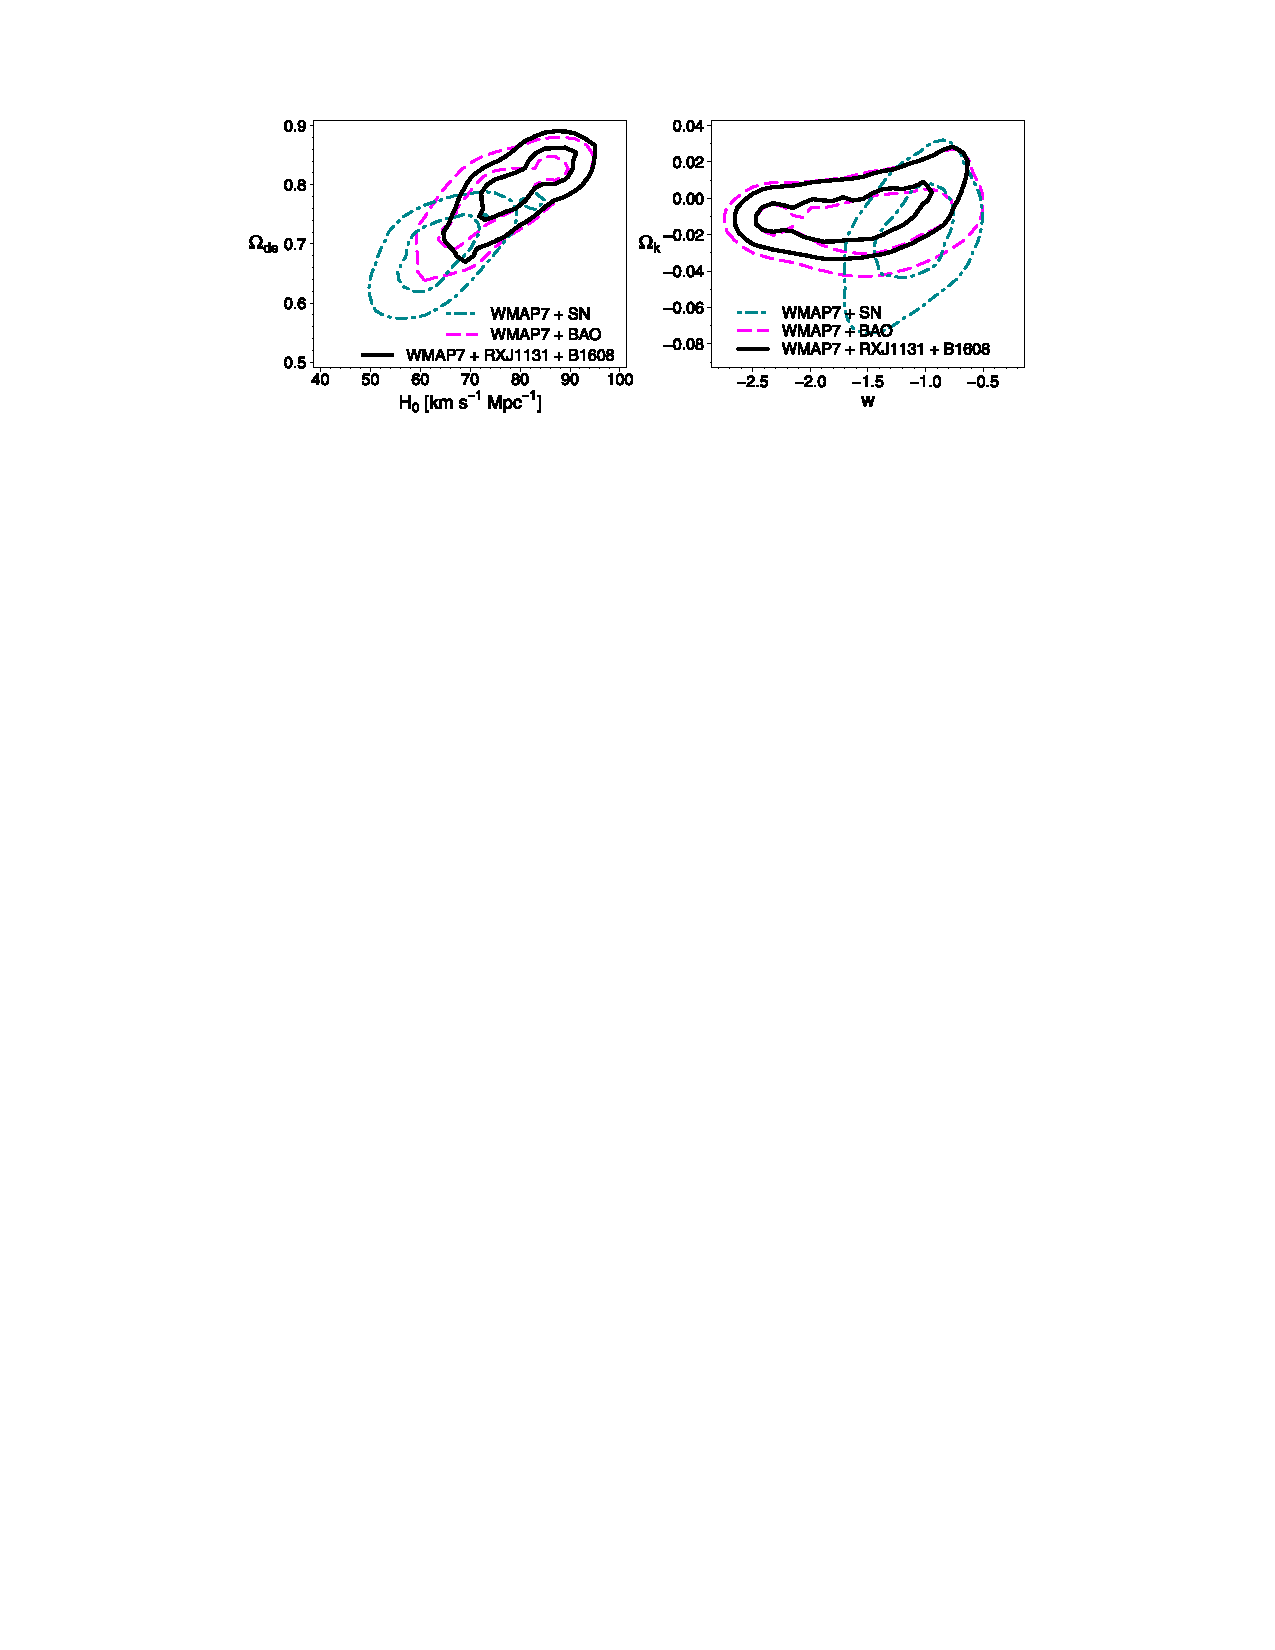
\includegraphics[width=0.9\linewidth]{figures/Suyu13_fig11.pdf}
\caption{Current cosmological parameter constraints from time delay
lenses. The marginalized posterior PDFs given the combined B1608$+$656
and RXJ1131 datasets and the assumption of an open CDM cosmology with
unknown dark energy equation of state is shown in
two sets of two parameter dimensions,
and compared to those given contemporary BAO and Type Ia supernova data.
Figure reproduced from \citet{Suy++14}.}
\label{fig:current-constraints}
\end{figure*}
%%%%%%%%%%%%%%%%%%%%%%%%%%%%%%%%%

While the sample of very well-measured lenses was being painstakingly
expanded from zero to two,  the exploration of statistical approaches to
dealing with large samples of lenses began. \citet{Ogu07b} \ldots simple model, doubles \ldots.
\citep{Rea++07} \ldots more flexible model, priors \ldots
\citet{RK++2015} \ldots towards hierarchical inference \ldots.
